\section{引言}
\label{sec:intro}
\blue{
时间序列预测支撑着气象服务~\citep{weathernature2025,wu2021autoformer}、能源规划~\citep{lai2018energy,alvarez2010energy,cheng2021windturbine}与交通管理~\citep{cirstea2022towardstraffic,cirstea2021enhancenet,wu2021autocts}中的决策。这些序列中有许多是时空的：它们由传感器网络产生，例如道路网络的环形线圈检测器或电网的智能电表。预测系统必须在每次更新时为网络中的每个传感器提供服务，因此效率与精度一样，都是一等要求~\citep{lai2023lightcts}。通道独立模型在设计上天然满足网络规模下的这一要求：一个共享模型分别且并行地预测每个传感器的序列~\citep{nie2023patchtst,zeng2023dlinear}，无需像基于图的模型那样在每次更新时收集并对齐相互连接的传感器的读数~\citep{wu2019graphwavenet}。其开销是每个传感器的计算量乘以传感器数量，因此每个传感器节省的每一次运算，都会在网络中每个传感器上、每次更新时各节省一次，而少量参数让共享模型在存储与重新训练上都保持低廉。

然而，预测模型正变得日益复杂。分解模型将序列拆分为趋势与季节性部分，并为每个部分配备专属网络~\citep{wu2021autoformer,zhou2022fedformer}；TimeMixer~\citep{timemixer24} 在多个尺度上分解序列并跨尺度混合各部分；TimesNet~\citep{wu2023timesnet} 同时建模多个周期；基于分块的 Transformer 将序列切分为连续取值的分块，并用深层注意力堆栈处理它们~\citep{nie2023patchtst,zhang2023crossformer}。在 Traffic 上，PatchTST~\citep{nie2023patchtst} 拥有 7.6M 参数量，其每次预测的 FLOPs 超出下文所提出的模型约 36,000 倍。\emph{预测周期性传感器数据流真的需要如此复杂吗？}我们表明并不需要。这些机制大多是为了解开标记所混合在一起的东西：当一个标记混杂多种信息时，网络必须学会将它们分离，并为此付出参数量与计算的代价。预测模型所需的能力，与其说取决于序列，不如说取决于其标记。若标记设计得当，极小的模型便已足够，而模型设计在很大程度上便成为标记设计。
}

\begin{figure*}[t]
  \centering
  \begin{subfigure}[t]{0.49\textwidth}
    \centering
    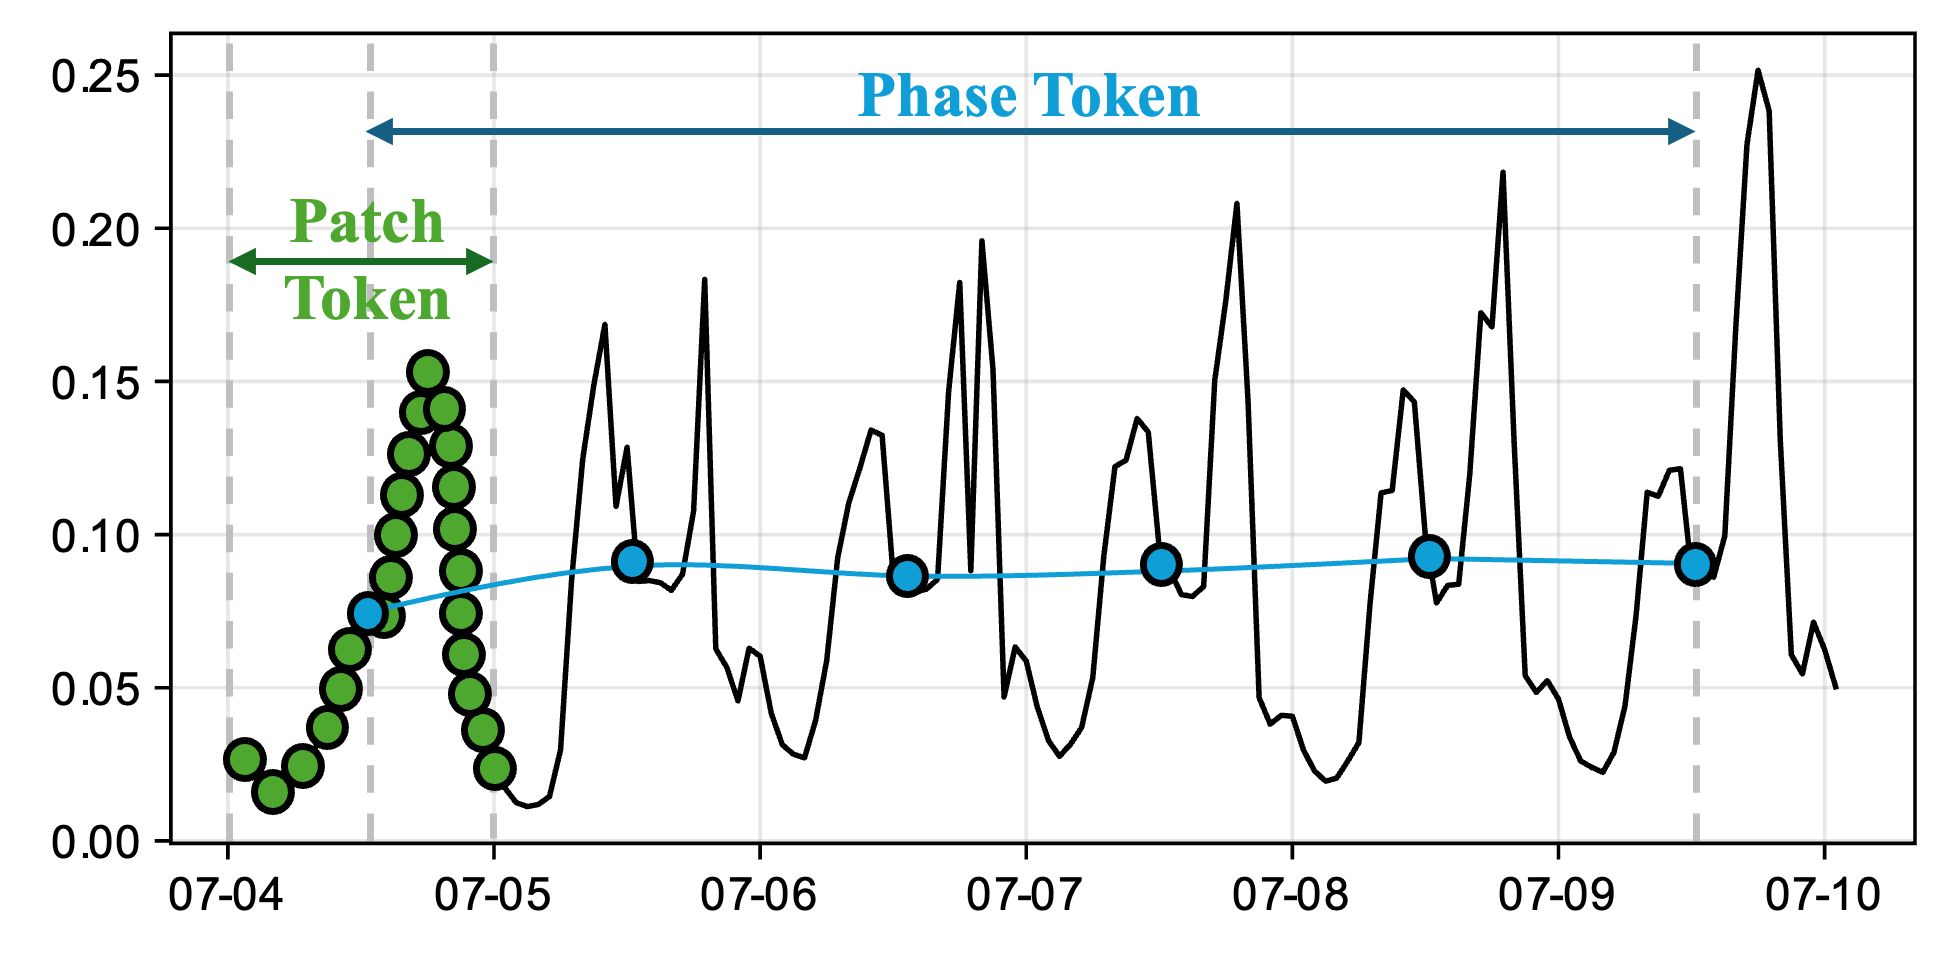
\includegraphics[width=\linewidth]{figures/phase_token.png}
    \caption{\blue{分块标记与相位标记。}}
    \label{fig:phase_token}
  \end{subfigure}
  \hfill
  \begin{subfigure}[t]{0.49\textwidth}
    \centering
    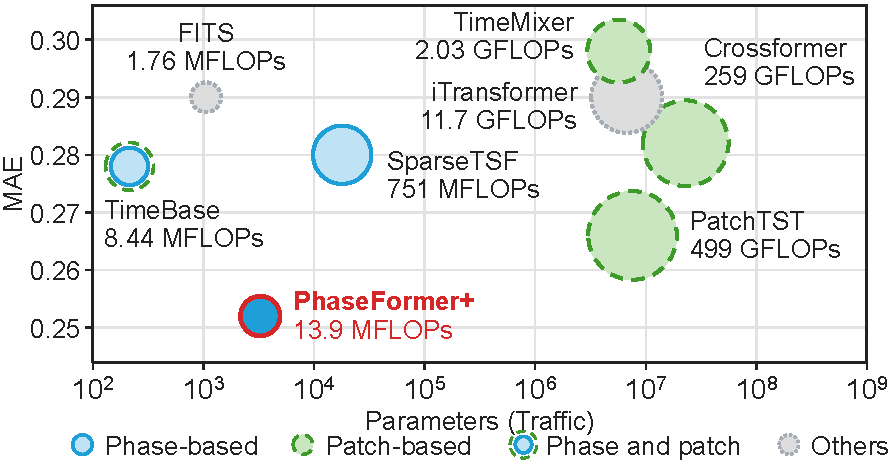
\includegraphics[width=\linewidth]{figures/efficiency_plot.pdf}
    \caption{\blue{精度与效率。}}
    \label{fig:efficiency_plot}
  \end{subfigure}
  \caption{\blue{好的标记让极小的模型便已足够。(a)~分块标记保存连续取值，即其所在周期在当前水平与振幅下的一段周期形状；相位标记收集相继各周期中同一相位处的取值。(b)~Traffic 上的精度与开销：四个预测时域上的平均 MAE 对预测时域 96（输入长度 720）时的参数量绘制；圆点大小随每次预测的 FLOPs 按对数增长，FLOPs 数值印在各名称下方。\sysplus 绘制时计入其相位通路以及水平与振幅通路至多约 2.1K 的参数量，其 FLOPs 取相位通路之值，水平与振幅通路对它增加不足 0.25\%。结合分块与相位的 TimeBase 以双圈标示；FEDformer（MAE 0.400）位于绘图范围之外。}}
  \label{fig:introduction}
\end{figure*}

\blue{
\fakeparagraph{标记应当表示什么}
标记是模型切分序列并在其上进行计算的基本单元，因此标记表示什么，决定了模型必须解开什么。那么，周期序列的标记应当表示什么？将窗口折叠成矩阵 $X$，每个周期一行，周期内每个位置一列，该位置称为其\emph{相位}。周期性意味着各行重复同一个模式，所以窗口首先包含的就是这个模式，即\emph{形状}，例如早高峰与晚高峰。然而重复从不精确，每个周期会在两个方面偏离共同的模式：它处在自己的高度上，即\emph{水平}（一个周期的均值），逐周期漂移，例如某条道路的交通量随周数增长；它还围绕这一水平摆动自己的幅度，即\emph{振幅}，且振幅随水平变动，例如更繁忙的日子里日负荷摆动得更宽。

这三者并不是随意列出的几个特征，而是关于一个重复周期所能说的全部内容：它长什么样、处在哪里、摆动多大。任何一个向量都等于它的均值加上一个尺度乘以一个方向。这里的方向是各周期共有的形状，均值与尺度则是周期之间不同的水平与振幅。就整个窗口而言，这就是一个紧凑结构：一个水平项加一个按振幅缩放的形状，$X\approx\ell\,\one^\top+a\,s^\top$，其中 $\ell$ 为各周期水平，$a$ 为各周期振幅，$s$ 为周期形状。数据印证了这一划分：这一秩二的单一形式在全部七个基准数据集上捕获了归一化输入窗口能量的 78\% 至 93\%（第\ref{sec:mot_tokens}节和图\ref{fig:token_energy}）。各部分占比有所不同：按振幅缩放的形状在 Electricity、Traffic 和 ETTh1 上承载大部分能量，水平则在其余四个数据集上占主导，因此任何一部分都不可省略。周期性窗口整体上是低维的，其每个部分亦然：$X$ 的各列张成一个平面，未来水平是平滑预测时域轮廓的少数几个系数，振幅是跟随水平的每周期一个因子。

现有的主流标记与这一结构并不吻合。分块标记保存连续取值，即其所在周期在当前水平与振幅下的一段周期形状，因此三者中任何一个变化，它都会变化：当通勤习惯改变而交通高峰移动时~\citep{shao2025hutformer,shao2025hyperd,zhou2025feddis}，当水平漂移时，或当繁忙的一天摆动更宽时。要覆盖这一宽泛且不断移动的标记分布，需要更大的表示，这会同时推高参数量与计算量~\citep{shao2025blast}：在 Traffic 上，前两个主成分可解释相位标记 74\% 的方差，而对分块标记只能解释 58\%（第\ref{sec:mot_stability}节）。

\fakeparagraph{为什么部分覆盖并不足够}
三类信息中的每一类与模型相遇，只有三种方式：由一个标记表示它；由标记把它与其他信息混在一起；或者没有任何标记携带它。留下混杂的部分落到网络上，网络必须学会把它解开，因此必须变大；遗漏的内容则丢失，精度随之受损。所以，标记只覆盖三类信息中的一部分的模型，必然要在容量与精度之间付出其中一种代价，无法回避这一选择。这是由部分覆盖本身推出的，而与任何具体模型的细节无关，现有模型也确实分别做出了这两种选择。Autoformer、FEDformer 和 TimeMixer 通过季节部分覆盖形状，并通过趋势覆盖部分水平——趋势是序列的平滑版本，而非逐周期的一个水平——但没有任何机制将季节性摆动与趋势绑定：一个摆动更宽的更繁忙的日子，到达季节性模型时已是一个新的季节性模式；而为每个部分配备的网络（TimeMixer 中还在多个尺度上配备）必须吸收拆分后残留的混合。TimesNet 按其多个周期折叠序列，与我们按单一周期折叠颇为相似，但它把每一折都交给一个深层卷积主干，后者必须自行从形状中分离出水平与振幅，且要同时应对多个周期；而一旦水平与振幅被表示出来，单一周期就已承载窗口能量的 78\% 至 93\%。基于分块的 Transformer 则把三者在每个分块标记中混杂地带入深层注意力堆叠。这些模型选择了容量：标记留下的混杂部分，要用参数量和计算量来偿付。DLinear、FITS 和 SparseTSF 等轻量模型选择了另一侧，保持小规模，但线性映射以同一组权重读取窗口的水平与形状，因此无法让在窗口上平均的形状按由近期周期预测出的水平缩放——这是对窗口两种不同读取之积——而 FITS 与 SparseTSF 在两个传感器网络 Electricity 和 Traffic 上落后（第\ref{sec:exp_results}节）。这些模型无一例外地只覆盖了三类信息的一部分，因而都落在容量与精度的权衡曲线上的某一点（第\ref{sec:related}节）。只有标记覆盖了全部三类，模型才可能在各基准数据集上既很小又准确，而一旦覆盖，留给网络去解开的便所剩无几。

\fakeparagraph{三个标记}
因此我们用三个标记表示一个窗口，每类信息一个，各自取该信息所具有的形式。\emph{相位标记}收集相继各周期中同一相位处的取值，即折叠矩阵的一列（图\ref{fig:phase_token}）；相位标记合起来承载形状。\emph{水平标记}是窗口各周期均值的向量，以最后一个观测值为基准；它承载水平，每周期一个数。\emph{振幅标记}是未来周期形状所按其缩放的因子；由于振幅跟随水平，它由水平标记计算，不需要自己的输入。这一划分源于每类信息各自的变化方式。按上述形式，相位 $p$ 处的相位标记为 $\ell+s_p\,a$：以形状加权的窗口水平与振幅轨迹。当一个窗口的每个周期以相同方式重塑时——例如每天早高峰都提前一小时——只有权重 $s_p$ 变化，因此相位标记在噪声范围内继续张成同一个低维子空间，而分块标记一般会移动到一个新的子空间（定理\ref{thm:stability}），这与 Traffic 上更紧凑的相位标记相一致。相反，水平或振幅的变化会改变 $\ell$ 或 $a$ 本身，从而移动该子空间（第\ref{sec:mot_changes}节）。相位标记因此是形状的稳定载体，而水平与振幅则在其沿周期变化之处被表示。

\fakeparagraph{\sysplus}
在这些标记之上，我们构建了 \textbf{\sysplus}：一个每个标记配一条小通路的预测模型（第\ref{sec:method}节）。\emph{相位通路}将相位标记嵌入一个共享的低维空间，让它们通过少量可学习的标记——路由器——交换信息，其代价随相位数量线性增长，并用一个共享预测器预测每个相位。\emph{水平通路}将水平标记映射到预测时域上的三个固定轮廓：一个偏移、一个倾斜和一个曲率；它绕过相位通路的各层归一化，因此它预测的水平不受其约束，下文的包络将这一点说得更精确。\emph{振幅通路}用由水平计算的因子重新缩放相位表示的周期内部分；由于这一缩放在各相位上中心化，它可证明地保持每个未来周期均值不变，因此振幅通路绝不会移动水平通路所设定的水平。两个门控融合相位与水平预测，一个用于周期水平，一个用于周期内形状。

\fakeparagraph{统一的低维视角}
三个标记并非三个彼此独立的装置。它们是窗口单一低维形式的三个因子，$X\approx\ell\,\one^\top+a\,s^\top$，而每条通路都取其因子的低维形式（第\ref{sec:theory}节）：相位通路预测形状 $s$，水平通路通过少数几个轮廓系数预测水平项，振幅通路通过水平预测因子 $a$。理论确立了这一对应关系的两半。第一，水平与振幅需要各自专属的通路。相位标记包含水平与振幅的轨迹，且相位通路具有足够表达能力：以合适的权重，它能实现 Holt--Winters 型的季节性预测模型~\citep{winters1960forecasting}，跟随水平漂移。然而对任意固定权重，其预测器读取的是层归一化的输出，即一个大小有界的向量，因此预测水平停留在一个固定区间内，周期内振幅低于一个固定上界。这些\emph{水平包络}与\emph{振幅包络}可由权重计算得到，需要超出包络的窗口会遭遇误差下界。更多深度、更多路由器或更多注意力头都无法消除它们：附加容量不能替代缺失的标记。

第二，包络之外的部分本身也是低维的。在标准季节性模型下，缺失的水平是每窗口少数几个数，各自乘以一个固定的预测时域轮廓；缺失的振幅是由水平驱动的一个因子缩放的周期形状；这些恰好是水平通路与振幅通路的形式。训练后的模型印证了这一点。要在每个窗口上追踪最近一个周期的水平，所需的水平包络会宽于训练权重在任何基准数据集上发展出的包络；而水平包络恰在 ETTh2、ETTm2 和 Weather 上约束生效，那里 12\% 至 21\% 的测试窗口需要包络之外的水平——这些正是水平标记收益最大的数据集。在 ETTh1 上，振幅包络约束生效而水平包络几乎不生效，带来收益的是振幅标记（第\ref{sec:exp_theory}节和第\ref{sec:exp_ladder}节）。

\fakeparagraph{结果}
\sysplus 在七个基准数据集中的六个上取得了相对八个基线的最佳平均 MSE（FITS 在 ETTh2 上领先），同时比基于分块的 Transformer 小若干个数量级。其优势为：在 Electricity 上领先 iTransformer 3.6\%，在两个传感器网络上领先小型跨周期预测模型 SparseTSF~\citep{lin2024sparsetsf} 与 TimeBase~\citep{huang2025timebase} 约 5\% 至 6\%（第\ref{sec:exp_results}节）。每个标记都名副其实：在同一训练协议下的标记消融中，\sysplus 在七个数据集均值中的五个上优于其仅相位变体，幅度最高达 3.3\%，在其余两个上与之相差不超过 0.3\%；其四项最大收益恰落在四个包络约束生效的数据集上（第\ref{sec:exp_ladder}节）。在最大的基准数据集 Traffic 上，相位通路需要约 1.2K 参数量，并将 PatchTST 和 Crossformer 的 FLOPs 削减约 99.99\%；水平与振幅通路至多增加约 2.1K 参数量，其中大部分是逐通道门控，在 Traffic 和 Electricity 上增加的 FLOPs 不足 0.25\%（图\ref{fig:efficiency_plot}与第\ref{sec:exp_efficiency}节）。预测周期性传感器数据流因此并不需要现有模型的复杂性：有了覆盖形状、水平与振幅的标记，几千参数量的模型便已足够；而由于一个共享模型服务每个传感器，计算上的每一点节省都会在网络每个传感器上、每次更新时重复兑现。

我们做出四项贡献：
\begin{enumerate}[leftmargin=2em]
\item \emph{以标记为中心的预测模型设计原则。}我们表明，周期序列的一个窗口携带三类信息——其各周期的形状、水平与振幅——它们构成一个秩二结构，在七个基准数据集上捕获归一化窗口能量的 78\% 至 93\%，且在其中五个数据集上振幅与水平相耦合。当标记覆盖全部三类信息时，预测模型既小又精确（第\ref{sec:motivations}节）。

\item \emph{\sysplus。}我们设计遵循这一结构的相位、水平与振幅标记，并各用一条小通路处理：一条跨相位路由并配共享预测器的相位通路，一条将水平标记映射到固定预测时域轮廓的水平通路，以及一条用水平重新缩放周期形状、且可证明地保持每个未来周期均值不变的振幅通路（第\ref{sec:method}节）。

\item \emph{三个标记的统一低维视角。}我们证明：当每个周期以相同方式重塑时，相位标记持续张成一个固定子空间，而分块标记一般不会；对固定权重，相位通路将预测水平与振幅限制在两个可由权重计算的包络内，超出包络则误差存在一个任何附加深度、路由器或注意力头都无法消除的下界；并且在标准季节性模型下，包络之外的部分恰好取水平通路与振幅通路的低维形式（第\ref{sec:mot_stability}节和第\ref{sec:theory}节）。

\item \emph{好标记胜过附加复杂性的证据。}以相位通路约 1.2K 参数量、水平与振幅至多再加约 2.1K 参数量，\sysplus 在七个基准数据集中的六个上取得了相对八个基线的最佳平均 MSE。在同一协议下逐个标记构建，它在七个数据集中的五个上取得收益，而从训练权重读出的包络恰好定位了水平标记收益最大的数据集（第\ref{sec:exp}节）。
\end{enumerate}

\fakeparagraph{与会议版本的关系}
本文是我们会议论文~\citep{niu2026phaseformer}的扩展版本，后者引入了相位标记与相位通路。水平与振幅标记、它们的通路、三个标记的统一低维视角（第\ref{sec:mot_tokens}节、第\ref{sec:mot_changes}节与第\ref{sec:theory}节），以及检验它们的实验，均为新增内容。
}
